\section{APOD}
\begin{frame}[fragile]
  \frametitle{APOD}
\begin{itemize}
\item ``CUDA Best Practices'' suggests \mydef{APOD} design cycle approach to cudarize your program.
\item \mydef{APOD -  Assess, Parallelize, Optimize, Deploy}
\item \mydef{Assess} - find the parts of the application where most of the time is spent, possibly using profiler. Use Amdahl's and Gustafson's laws to understand expected performance benefits from parallelizing that part of the code.
\item \mydef{Parallelize} - parallelize the identified bottleneck. Perhaps use the existing library such as 
  cuBLAS, cuFFT, cuSPARSE, Thrust, etc. Or write it from scratch in CUDA.
\item \mydef{Optimize} - optimize the parallel version using your understanding of the underlying hardware
\item \mydef{Deploy} - put it in production ASAP. This would allow to identify potential problems and benefit from the achieved performance gain faster
\end{itemize}
\end{frame}


\begin{frame}[fragile]
  \frametitle{APOD}
\begin{itemize}
\item APOD is a cyclical process: initial speedups can be achieved, tested, and deployed with
  only minimal initial investment of time, at which point the cycle can begin again by
  identifying further optimization opportunities, seeing additional speedups, and then
  deploying the even faster versions of the application into production.
\end{itemize}
\begin{center}
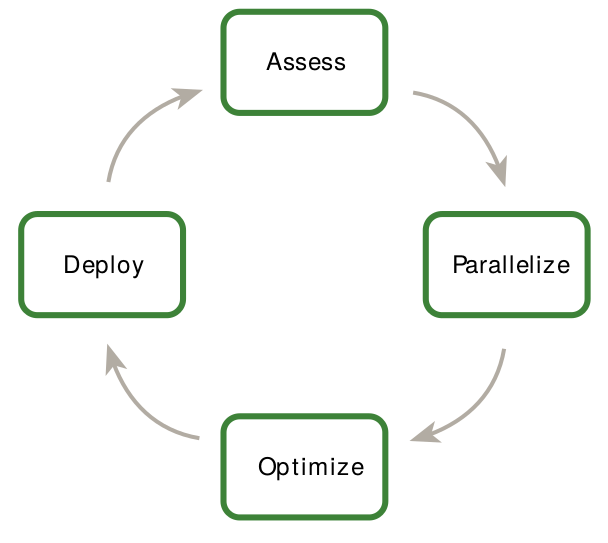
\includegraphics[width=5.0cm]{graphs/apod.png}
\end{center}
\end{frame}